\section{Đề ôn thi giữa kỳ 2 toán 11}
\subsection{Phần trắc nghiệm}
Câu trắc nghiệm nhiều phương án lựa chọn. Học sinh trả lời từ
câu 1 đến câu 12. Mỗi câu hỏi học sinh \textit{chỉ chọn một} phương án.

\Opensolutionfile{ans}[Ans/Dapan]

\hienthiloigiaiex
%%%=============EX_1=============%%%
\begin{ex}%[1D6N1-2]%[Dự án đề kiểm tra Toán khối 11 GHKII NH3-24-Dot2-Nguyễn Văn Hiệp]%[Deso2-Phan Nhật Linh]
	Với $\alpha$ là một số thực bất kỳ, mệnh đề nào sau đây \textbf{sai}?
	\choice
	{$\sqrt{10^{\alpha}}=\left(\sqrt{10}\right)^{\alpha}$}
	{\True $\left(10^{\alpha}\right)^2=10^{\alpha^2}$}
	{$\left(10^{\alpha}\right)^{2}=(100)^{\alpha}$}
	{$\sqrt{10^{\alpha}}=10^{\tfrac{\alpha}{2}}$}
	\loigiai{$\left(10^{\alpha}\right)^2=10^{\alpha^2}$ sai vì $\left(10^{\alpha}\right)^2=10^{2\alpha}$.}
\end{ex}
%%%=============EX_2=============%%%
\begin{ex}%[1D6N1-2]%[Dự án đề kiểm tra Toán khối 11 GHKII NH3-24-Dot2-Nguyễn Văn Hiệp]%[Deso2-Phan Nhật Linh]
	Cho $a$ là số thực dương và $m$, $n$ là các số thực tùy ý. Trong các tính chất sau tính chất nào \textbf{sai}?
	\choice
	{\True $a^m \cdot b^n=(a b)^{m+n}$}
	{$a^{m-n}=\dfrac{a^m}{a^n}$}
	{$a^{m+n}=a^m \cdot a^n$}
	{$a^{m \cdot n}=\left(a^n\right)^m$}
	\loigiai{Với $m=2$; $n=3$ thì $a^m \cdot b^n=a^2 b^3$; $(a b)^{m+n}=(ab)^5=a^5b^5$.}
\end{ex}
%%%=============EX_3=============%%%
\begin{ex}%[1H8H1-3]%[Dự án đề kiểm tra Toán khối 11 GHKII NH3-24-Dot2-Nguyễn Văn Hiệp]%[Deso2-Phan Nhật Linh]
	Cho hình lập phương $A B C D .A^{\prime}B^{\prime}C^{\prime}D^{\prime}$. Góc giữa hai đường thẳng $A A^{\prime}$ và $B D$ bằng bao nhiêu độ?
	\choice
	{$30^\circ$}
	{$60^\circ$}
	{$45^\circ$}
	{\True $90^\circ$}
	\loigiai{\immini{Do $AA' \perp (ABCD)$ suy ra $AA' \perp BD$ nên $\left(AA',BD\right)=90^\circ$.}{
			\begin{tikzpicture}[line join=round, line cap=round,>=stealth,scale=0.8]
				\def\a{3.5}
				\path 	(0:0) coordinate (A)
				++(0:\a) coordinate (D)
				++(-130:\a/2) coordinate (C)
				($(A)+(C)-(D)$) coordinate (B)
				($(A)+(90:\a)$) coordinate (A')
				($(B)+(90:\a)$) coordinate (B')
				($(C)+(90:\a)$) coordinate (C')
				($(D)+(90:\a)$) coordinate (D');
				\draw[dashed,thick] 	(B)--(A)--(D)	(A)--(A');
				\draw[thick] 	(C)--(C') 	(D)--(D') 	(B)--(B') 	(B)--(C)--(D) (A')--(B')--(C')--(D')--cycle;
				\foreach \x/\g in {A/180,B/180,C/0,D/0,A'/180,B'/180,C'/0,D'/0}
				\fill[black] 	(\x) circle (1pt)
				($(\g:4mm)+(\x)$) node {$\x$};	
	\end{tikzpicture}}}
\end{ex}
%%%=============EX_4=============%%%
\begin{ex}%[1H8H2-1]%[Dự án đề kiểm tra Toán khối 11 GHKII NH3-24-Dot2-Nguyễn Văn Hiệp]%[Deso2-Phan Nhật Linh]
	Trong không gian cho hai đường thẳng phân biệt $a$; $b$ và mặt phẳng $(P)$, trong đó $a \perp(P)$. Mệnh đề nào sau đây \textbf{sai}?
	\choice
	{Nếu $b \parallel a$ thì $b \perp(P)$}
	{\True Nếu $b \perp a$ thì $b \parallel (P)$}
	{Nếu $b \parallel (P)$ thì $b \perp a$}
	{Nếu $b \perp(P)$ thì $b \parallel a$}
	\loigiai{Nếu $b\subset (P)$ thì $b\perp a$.}
\end{ex}
%%%=============EX_5=============%%%
\begin{ex}%[1H8N6-1]%[Dự án đề kiểm tra Toán khối 11 GHKII NH3-24-Dot2-Nguyễn Văn Hiệp]%[Deso2-Phan Nhật Linh]
	Cho hình chóp $S.A B C$ có cạnh bên $S A$ vuông góc mặt đáy $(A B C)$. Góc tạo bởi $S B$ và đáy tương ứng là
	\choice
	{$\widehat{SCA}$}
	{\True $\widehat{SBA}$}
	{$\widehat{SBC}$}
	{$\widehat{SAB}$}
	\loigiai{\immini{Do $SA\perp (ABC)$ nên $\left(SB,(ABC)\right)=(SB,AB)=\widehat{SBA}$.}{\begin{tikzpicture}[line join=round, line cap=round,>=stealth,scale=0.8]
				\def\a{4} %Khai báo cạnh
				\def\h{4}
				\path 	(0:0) coordinate (A)
				++(0:\a) coordinate (B)
				++(-150:4*\a/5) coordinate (C)
				($(A)+(90:\h)$) coordinate (S)
				($(A)!0.5!(B)$) coordinate (M);
				\draw[thick] 	(A)--(C)--(B)
				(A)--(S)	(B)--(S)	(C)--(S);
				\draw[dashed,thick] 	(A)--(B);
				\foreach \x /\goc in {A/180,B/0,C/-135,S/90}
				\fill[black] (\x) circle (0pt)
				($(\x)+(\goc:3mm)$) node {$\x$};
				\draw pic[draw,angle radius=2mm]{right angle=B--A--S};%Theo chiều dương
		\end{tikzpicture}}
	}
\end{ex}
%%%=============EX_6=============%%%
\begin{ex}%[1D6H1-2]%[Dự án đề kiểm tra Toán khối 11 GHKII NH3-24-Dot2-Nguyễn Văn Hiệp]%[Deso2-Phan Nhật Linh]
	Với $a$ là số thực dương tùy ý, $\sqrt[3]{a^2}$ bằng
	\choice
	{$a^{\tfrac{1}{6}}$}
	{$a^6$}
	{\True $a^{\tfrac{2}{3}}$}
	{$a^{\tfrac{3}{2}}$}
	\loigiai{$\sqrt[3]{a^2}=a^{\tfrac{2}{3}}$.}
\end{ex}
%%%=============EX_7=============%%%
\begin{ex}%[1D6H3-4]%[Dự án đề kiểm tra Toán khối 11 GHKII NH3-24-Dot2-Nguyễn Văn Hiệp]%[Deso2-Phan Nhật Linh]
	Cho $a, b>0$ thỏa mãn $a^{\tfrac{2}{3}}>a^{\tfrac{1}{2}}$, $b^{\tfrac{2}{3}}>b^{\tfrac{3}{4}}$. Khi đó khẳng định nào sau đây đúng?
	\choice
	{$0<a<1$, $b>1$}
	{\True $a>1$, $0<b<1$}
	{$a>1$, $b>1$}
	{$0<a<1$, $0<b<1$}
	\loigiai{
		\begin{itemize}
			\item $a^{\tfrac{2}{3}}>a^{\tfrac{1}{2}}\Leftrightarrow \dfrac{2}{3}> \dfrac{1}{2}$ suy ra $a>1$.
			\item $b^{\tfrac{2}{3}}>b^{\tfrac{3}{4}}\Leftrightarrow \dfrac{2}{3}<\dfrac{3}{4}$ suy ra $0<b<1$.
		\end{itemize}
	}
\end{ex}
%%%=============EX_8=============%%%
\begin{ex}%[1D6H2-1]%[Dự án đề kiểm tra Toán khối 11 GHKII NH3-24-Dot2-Nguyễn Văn Hiệp]%[Deso2-Phan Nhật Linh]
	Cho $a, b$ là các số thực dương, $a \neq 1$ thỏa mãn $\log _{a}b=3$. Tính $\log _{\sqrt{a}}a^2b^3$.
	\choice
	{$24$}
	{$25$}
	{\True $22$}
	{$23$}
	\loigiai{\allowdisplaybreaks
		\begin{eqnarray*}
			\log _{\sqrt{a}}a^2b^3&=&\log _{a^{\tfrac{1}{2}}}a^2b^3\\
			&=&2\log_a \left(a^2b^3\right)\\
			&=&2\left(\log_a a^2+\log_a b^3\right)\\
			&=&2\left(2+3\log_a b\right)\\
			&=&22.
		\end{eqnarray*}
	}
\end{ex}
%%%=============EX_9=============%%%
\begin{ex}%[1H8H2-1]%[Dự án đề kiểm tra Toán khối 11 GHKII NH3-24-Dot2-Nguyễn Văn Hiệp]%[Deso2-Phan Nhật Linh]
	Cho hai đường thẳng $a$, $b$ và mặt phẳng $(P)$. Trong các mệnh đề sau mệnh đề nào \textbf{sai}?
	\choice
	{Nếu $a \perp(P)$ và $b \perp a$ thì $b \parallel (P)$ hoặc $b \subset(P)$}
	{\True Nếu $a \parallel (P)$ và $b \perp a$ thì $b \perp(P)$}
	{Nếu $a \parallel (P)$ và $b \perp(P)$ thì $a \perp b$}
	{Nếu $a \subset(P)$ và $b \perp(P)$ thì $a \perp b$}
	\loigiai{Nếu $a \parallel (P)$ và $b \perp a$ thì $b \perp(P)$
		là sai vì có thể có $b\subset (P)$ và $b\perp a$.
	}
\end{ex}
%%%=============EX_10=============%%%
\begin{ex}%[1D6H1-3]%[Dự án đề kiểm tra Toán khối 11 GHKII NH3-24-Dot2-Nguyễn Văn Hiệp]%[Deso2-Phan Nhật Linh]
	Tập xác định của hàm số $y=(x-1)^{\sqrt{3}}$ là
	\choice
	{$\mathbb{R}\setminus \{1\}$}
	{$\mathbb{R}$}
	{\True $(1 ;+\infty)$}
	{$(-1 ;+\infty)$}
	\loigiai{Do $\sqrt{3}\in \mathbb{I}$ nên điều kiện xác định $x-1>0\Leftrightarrow x>1$. Vậy $\mathscr{D}=(1 ;+\infty)$.}
\end{ex}
%%%=============EX_11=============%%%
\begin{ex}%[1D6H3-3]%[Dự án đề kiểm tra Toán khối 11 GHKII NH3-24-Dot2-Nguyễn Văn Hiệp]%[Deso2-Phan Nhật Linh]
	\immini{Đường cong trong hình bên là của đồ thị hàm số nào sau đây?	}{\begin{tikzpicture}[line join=round, line cap=round,>=stealth,thick,scale=0.7]
			\tikzset{every node/.style={scale=0.9}}
			\draw[->] (-5.5,0)--(5,0) node[below left] {$x$};
			\draw[->] (0,-0.6)--(0,4) node[below left] {$y$};
			\draw (0,0) node [below left] {$O$};
			\begin{scope}
				\clip (-5,-0.5) rectangle (5,5);
				\draw[samples=200,domain=-5:4.5,smooth,variable=\x] plot (\x,{(0.8)^(\x)});
			\end{scope}
	\end{tikzpicture}}
	\choice
	{$y=\log _{2}x$}
	{\True $y=(0{,}8)^{x}$}
	{$y=\log _{0{,}4}x$}
	{$y=(\sqrt{2})^{x}$}
	\loigiai{Đồ thị hàm số nằm phía trên trục hoành và hàm số nghịch biến nên đường cong là đồ thị hàm số $y=(0{,}8)^{x}$.}
\end{ex}
%%%=============EX_12=============%%%
\begin{ex}%[1D6H3-4]%[Dự án đề kiểm tra Toán khối 11 GHKII NH3-24-Dot2-Nguyễn Văn Hiệp]%[Deso2-Phan Nhật Linh]
	Trong các khẳng định sau, khẳng định nào \textbf{sai}?
	\choice
	{$\log _{a^2+4}\left(a^2+1\right) \ge 0$, $\forall a$}
	{$4^{-\sqrt{3}}<4^{-\sqrt{2}}$}
	{$2^{30}<3^{20}$}
	{\True $0{,}99^{\pi}>0{,}99^{\mathrm{e}}$}
	\loigiai{Do hàm số $y=0{,}99^x$ nghịch biến trên $\mathbb{R}$ và $\pi > \mathrm{e}$ nên $0{,}99^{\pi}<0{,}99^{\mathrm{e}}$.}
\end{ex}

\Closesolutionfile{ans}
\bangdapan{Dapan}

\subsection{Câu trắc nghiệm đúng sai}
Học sinh trả lời từ câu 1 đến câu 4.
Trong mỗi ý \circlenum{A}, \circlenum{B}, \circlenum{C} và \circlenum{D} ở mỗi câu, học sinh chọn đúng hoặc sai.
\setcounter{ex}{0}
\LGexTF
\Opensolutionfile{ansbook}[ansbook/DapanDS]
\Opensolutionfile{ans}[Ans/DapanT]
%%%============EX_1==============%%%

\begin{ex}%[1D6H3-3]
	Hình vẽ dưới đây là đồ thị của các hàm số mũ $y=a^x$, $y=b^x$, $y=c^x$.
	\begin{center}
		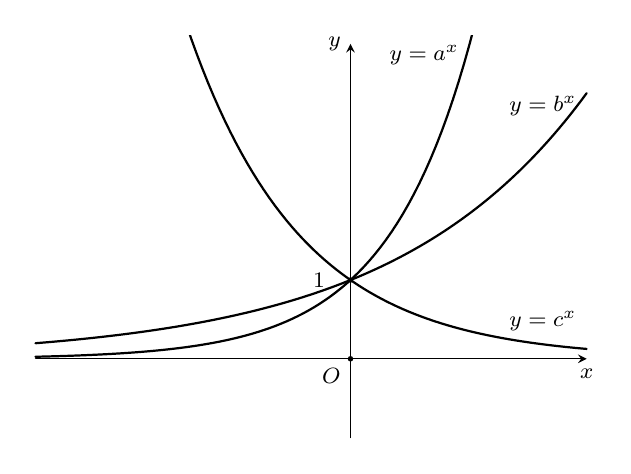
\begin{tikzpicture}[scale=1, font=\footnotesize, line join=round, line cap=round,>=stealth]%<DTools>
			%Gán số liệu.
			\def\xmin{-4};\def\ymin{-1};\def\xmax{3};\def\ymax{4};
			%Gán tọa độ.
			\coordinate (O) at (0,0);
			%Trục Oxy.
			\draw[->] (\xmin,0)--(\xmax,0) node[below]{$x$};
			\draw[->] (0,\ymin)--(0,\ymax) node[left]{$y$};
			\fill (O) node[below left]{$O$} circle(1pt);
			%Giới hạn đồ thị.
			\clip ({\xmin-0.1},{\ymin-0.1}) rectangle ({\xmax+0.1},{\ymax+0.1});
			\foreach \y in {1}{
				\fill (0,\y) node[left=2mm]{$\y$} circle(1pt);
			}
			%Vẽ đồ thị.
			\draw[thick,samples=100] plot[domain=-4:3](\x,{pow(1.5,(\x))}) node[below left=-1mm,xshift=-1mm] {$y=b^x$};
			\draw[thick,samples=100] plot[domain=-4:3](\x,{pow(2.5,(\x))});
			\path
			(1.5,{pow(2.5,1.5)}) node[left,yshift=-1mm] {$y=a^x$}
			;
			\draw[thick,samples=100] plot[domain=-4:3](\x,{pow(0.5,(\x))})
			node[above left=-1mm,xshift=-1mm,yshift=2mm] {$y=c^x$};
			
		\end{tikzpicture}
		
	\end{center}
	\choiceTF
	{Từ đồ thị, hàm số $y=a^x$ là hàm số nghịch biến}
	{Hàm số $y=c^x$ là hàm số nghịch biến nên $c<1$}
	{Hai hàm số $y=a^x$ và $y=b^x$ là hai hàm số đồng biến nên $a<b$}
	{Hai hàm số $y=a^x$ và $y=b^x$ là hai hàm số đồng biến và $y=c^x$ là hàm số nghịch biến nên ta suy ra được $a>b>1>c$}
	\loigiai
	{
		Từ đồ thị, hàm số $y=a^x$ là hàm số đồng biến.\\
		Hàm số $y=c^x$ là hàm số nghịch biến nên $0<c<1$.\\
		Hai hàm số $y=a^x$ và $y=b^x$ là hai hàm số đồng biến, không đủ điều kiện để kết luận $b<a$.\\
		Hai hàm số $y=a^x$ và $y=b^x$ là hai hàm số đồng biến và $y=c^x$ là hàm số nghịch biến, ta chỉ có thể suy ra $a$ và $b$ lớn 1 và $c<1$, không thể so sánh $a$ và $b$ dựa trên tính đồng biến của hàm số.
	}
\end{ex}

\begin{ex}%[1H8H2-2]%[1H8H4-3]
	Cho hình chóp $S. ABC$ có đáy là tam giác vuông cân tại $B$, $AB=BC=a$. Cạnh bên $SA$ vuông góc với mặt phẳng đáy $(ABC)$ và $SA=a$. Gọi $I$ là trung điểm của $AC$ và kẻ $IH\perp SC$.
	\begin{center}
		\begin{tikzpicture}[scale=1, font=\footnotesize,>=stealth]%<DTools>
			%Gán số liệu.
			\def\canhAC{4};\def\canhBA{2};\def\gocBAC{-45};\def\h{3};\def\xdinhS{0};
			%Gán tọa độ.
			\coordinate (A) at (0,0);
			\coordinate (B) at ($(A)+(\gocBAC:\canhBA)$);
			\coordinate (C) at ($(A)+(0:\canhAC)$);
			\coordinate (S) at ($(A)+(\xdinhS,\h)$);
			\path
			($(A)!.5!(C)$) coordinate (I)
			($(S)!(I)!(C)$) coordinate (H)
			
			;
			%Vẽ khối chóp S.ABC.
			\draw (S)--(B) (S)--(A)--(B) (S)--(C)--(B)--(H)
			\foreach \x/\y/\z in {C/B/A,I/H/C,C/A/S}{
				pic[draw, angle radius = 6pt]{right angle = \x--\y--\z}
			}
			
			;
			\draw[dashed] (A)--(C)  (I)--(H) (B)--(I);
			%Gán nhãn.
			\foreach \x/\y in {S/90,A/180,B/-90,C/0,I/90,H/45}{\fill (\x) circle (1pt) ($(\x)+(\y:0.3cm)$) node{$\x$};}
		\end{tikzpicture}
	\end{center}
	\choiceTF
	{\True Đường thẳng $SC$ vuông góc với mặt phẳng $(BHI)$}
	{Cosin góc tạo bởi hai đường thẳng $IH$ và $BH$ bằng $\dfrac{\sqrt{3}}{2}$}
	{Độ dài đoạn thẳng $BH$ bằng $\dfrac{a\sqrt{2}}{2}$}
	{\True Góc giữa hai mặt phẳng $(SAC)$ và $(SBC)$ bằng $60^\circ$}
	\loigiai
	{
		$\triangle ABC$ vuông cân tại $B$, $I$ là trung điểm của $AC$ nên $BI\perp AC$.\\
		Mà $SA\perp BI$ do $SA\perp (ABC)$ nên suy ra $BI\perp (SAC) \Rightarrow BI\perp SC$.\\
		Mà $SC\perp IH \Rightarrow SC\perp (BHI)$.\\
		Tam giác $BIH$ vuông tại $I$ nên $\cos (IH;BH)=\dfrac{IH}{BH}$.\\
		Dễ thấy $AC=a\sqrt{2} \Rightarrow BI=\dfrac{AC}{2}=\dfrac{a\sqrt{2}}{2}$.\\
		$SC=\sqrt{SA^2+AC^2}=\sqrt{a^2+2a^2}=a\sqrt{3}$.\\
		$\triangle HIC \backsim \triangle ASC \Rightarrow \dfrac{IH}{SA}=\dfrac{IC}{SC}=\dfrac{\dfrac{a\sqrt{2}}{2}}{a\sqrt{3}}=\dfrac{1}{\sqrt{6}}\Rightarrow IH=\dfrac{1}{\sqrt{6}}\cdot SA=\dfrac{1}{\sqrt{6}}\cdot a$.\\
		$\tan \widehat{IHB}=\dfrac{IB}{IH}=\dfrac{\dfrac{a\sqrt{2}}{2}}{\dfrac{a}{\sqrt{6}}}=\sqrt{3}\Rightarrow \widehat{IHB}=60^\circ \Rightarrow \cos (IH;BH)=\dfrac{1}{2}$.\\
		$BH=\sqrt{IB^2+IH^2}=\sqrt{\dfrac{a^2}{2}+\dfrac{a^2}{6}}=\dfrac{a\sqrt{2}}{\sqrt{3}}=\dfrac{a\sqrt{6}}{3}$.\\
		Góc giữa hai mặt phẳng $(SAC)$ và $(SBC)$ là góc $\widehat{IHB}=60^\circ$.
	}
\end{ex}

\begin{ex}%[1D6V4-2]
	Cho phương trình $9^{x+1}-13\cdot 6^x+4^{x+1}=0$. Xét tính đúng sai của các mệnh đề sau
	\choiceTF
	{\True Nếu đặt $\left(\dfrac{3}{2}\right)^x=t$ thì phương trình đã cho trở thành $9t^2-13t+4=0$}
	{\True Phương trình đã cho có hai nghiệm, trong đó có một nghiệm nguyên âm}
	{Tổng tất cả các nghiệm của phương trình đã cho bằng 0}
	{Phương trình đã cho có hai nghiệm và đều là nghiệm nguyên dương}
	\loigiai
	{
		Ta có
		$\begin{aligned}[t]
			&9^{x+1}-13\cdot 6^x+4^{x+1}=0\\
			\Leftrightarrow~&9\cdot 9^x-13\cdot 6^x+4\cdot 4^x=0\\
			\Leftrightarrow~&9\cdot \dfrac{9^x}{4^x}-13\cdot \dfrac{3^x}{2^x}+4=0.\qquad(1)
		\end{aligned}$\\
		Đặt $\left(\dfrac{3}{2}\right)^x=t$  thì phương trình (1) trở thành $9t^2-13t+4=0.\qquad (2)$\\
		Phương trình (2) có hai nghiệm $t_1=1$ và $t_2=\dfrac{4}{9}$.\\
		Suy ra phương trình (1) có hai nghiệm $x_1=0$ và $x_2=-2$.\\
		Tổng các nghiệm của phương trình (1) là $x_1+x_2=0+(-2)=-2$.\\
		
	}
\end{ex}

\begin{ex}%[1H8H6-1]
	Cho hình chóp $S.ABC$ có đáy $ABC$ là tam giác đều cạnh $a$. Biết $SA=a\sqrt{2}$ và $SA$ vuông góc với mặt đáy. Gọi $M$ là trung điểm của $BC$ và $H$ là hình chiếu vuông góc của $A$ lên $SM$.
	\choiceTF
	{\True Đường thẳng $AH$ vuông góc với mặt phẳng $(SBC)$}
	{\True Đường thẳng $SH$ là hình chiếu của đường thẳng $SA$ lên mặt phẳng $(SBC)$}
	{Độ dài đoạn thẳng $AH$ bằng $\dfrac{6a}{11}$}
	{Cosin góc tạo bởi đường thẳng $SA$ và mặt phẳng $(SBC)$ bằng $\dfrac{\sqrt{11}}{33}$}
	\loigiai
	{
		\begin{center}
			\begin{tikzpicture}[scale=1, font=\footnotesize,>=stealth]%<DTools>
				%Gán số liệu.
				\def\canhAC{4};\def\canhBA{2};\def\gocBAC{-50};\def\h{3};\def\xdinhS{0};
				%Gán tọa độ.
				\coordinate (A) at (0,0);
				\coordinate (B) at ($(A)+(\gocBAC:\canhBA)$);
				\coordinate (C) at ($(A)+(0:\canhAC)$);
				\coordinate (S) at ($(A)+(\xdinhS,\h)$);
				\path
				($(C)!.5!(B)$) coordinate (M)
				($(S)!.4!(M)$) coordinate (H)
				
				;
				%Vẽ khối chóp S.ABC.
				\draw (S)--(B) (S)--(A)--(B) (S)--(C)--(B) (S)--(M)
				\foreach \x/\y/\z in {S/H/A,A/M/B}{
					pic[draw, angle radius = 6pt]{right angle = \x--\y--\z}
				}
				;
				\draw[dashed] (A)--(C) (M)--(A)--(H);
				%Gán nhãn.
				\foreach \x/\y in {S/90,A/180,B/-90,C/0,M/-60,H/60}{\fill (\x) circle (1pt) ($(\x)+(\y:0.3cm)$) node{$\x$};}
			\end{tikzpicture}
		\end{center}
		$BC\perp AM$ ($AM$ là đường trung tuyến trong tam giác đều $ABC$).\\
		Mà $SA\perp (ABC) \Rightarrow SA\perp BC$.\\
		Suy ra $BC\perp (SAM) \Rightarrow BC\perp AH$.\\
		Mà $AH\perp SM$ (theo đề bài) nên $AH\perp (SBC)\Rightarrow SH$ là hình chiếu của $SA$ lên mặt phẳng $(SBC)$.\\
		Xét tam giác vuông $SAM$ tại $A$ ta có
		$$
		\dfrac{1}{AH^2}=\dfrac{1}{SA^2}+\dfrac{1}{AM^2}=\dfrac{1}{2a^2}+\dfrac{1}{\dfrac{3a^2}{4}} \Rightarrow AH=\sqrt{\dfrac{6}{11}}a.
		$$
		Góc giữa $SA$ là mặt phẳng $(SBC)$ là góc $\widehat{ASM}$.\\
		Ta có $\tan \widehat{SAM}=\dfrac{AM}{SA}=\dfrac{\dfrac{a\sqrt{3}}{2}}{a\sqrt{2}}=\dfrac{\sqrt{3}}{2\sqrt{2}}=\dfrac{\sqrt{6}}{4}$.
	}
\end{ex}


\Closesolutionfile{ans}
\Closesolutionfile{ansbook}

\begin{center}
	\textbf{\textsf{BẢNG ĐÁP ÁN ĐÚNG SAI}}
\end{center}
\input{Ansbook/DapanDS}
\subsection{Phần tự luận}

\hienthiloigiaibt
%%%=============BT_1=============%%%
\begin{bt}%[1D6V2-2]%[Dự án đề kiểm tra Toán khối 10 GHKII NH23-24-Dot 2-Nguyễn Khánh Trọng]%[Deso2-Phan Nhật Linh]
	Cho các số thực dương $a$, $b$ thỏa mãn $\log_{16}a=\log_{20}b=\log_{25}\dfrac{2a-b}{3}$. Tính tỉ số $\dfrac{a}{b}$ (Kết quả viết dưới dạng thập phân).
	\loigiai{
		Đặt $\log_{16}a=\log_{20}b=\log_{25}\dfrac{2a-b}{3}=t$.\\
		Suy ra $\heva{&a=16^t\\&b=20^t\\&\dfrac{2a-b}{3}=25^t}\Rightarrow 2\cdot16^t-20^t=3\cdot25^t\Leftrightarrow 2\cdot\left(\dfrac{16}{25}\right)^t-\left(\dfrac{4}{5}\right)^t-3=0\Leftrightarrow \hoac{&\left(\dfrac{4}{5}\right)^t=\dfrac{3}{2}\\&\left(\dfrac{4}{5}\right)^t=-1 \text{ (vô lí).}}$\\
		Vậy $\dfrac{a}{b}=\dfrac{16^t}{20^t}=\left(\dfrac{4}{5}\right)^t=\dfrac{3}{2}=1{,}5$.
	}
\end{bt}

\begin{bt}%[1H8H1-3]%[Dự án đề kiểm tra Toán khối 10 GHKII NH23-24-Dot 2-Nguyễn Khánh Trọng]%[Deso2-Phan Nhật Linh]
	Cho tứ diện $ABCD$ có $AC = 6$; $BD = 8$ có $AC\perp BD$. Gọi $M$, $N$ lần lượt là trung điểm của $AD$, $BC$. Tính độ dài đoạn thẳng $MN$.
	\loigiai{
		\immini{
			Gọi $P$ là trung điểm của $AB$. \\
			Khi đó $MP\parallel BD$ và $NP\parallel AC\Rightarrow \left(MP,NP\right)=\left(BD,AC\right)=90^\circ$.\\
			Suy ra $MN=\sqrt{MP^2+NP^2}=\sqrt{\left(\dfrac{BD}{2}\right)^2+\left(\dfrac{AC}{2}\right)^2}=5$.
		}{\begin{tikzpicture}[line join=round,line cap=round,>=stealth,scale=0.75,font=\footnotesize]
			\foreach \x/\y/\n in {0/0/A,2/-2/B,6/0/C} \coordinate (\n) at (\x,\y);
			\coordinate (D) at ($(A)+(3,4)$); 
			\coordinate (M) at ($(A)!0.5!(D)$); 
			\coordinate (N) at ($(B)!0.5!(C)$); 
			\coordinate (P) at ($(B)!0.5!(A)$); 
			\foreach \t/\g in {A/180,B/-90,C/0,D/90,M/120,N/-60,P/-120}{
				\draw[fill=black] (\t) circle (1pt) node[shift={(\g:8pt)}]{$ \t $};
			\draw (D)--(A)--(B)--(C)--(D)--(B) (M)--(P);
			\draw[dashed] (A)--(C) (M)--(N)--(P);
			\draw pic[thin,draw,angle radius=2mm] {right angle= M--P--N};
			}
		\end{tikzpicture}}
	}
\end{bt}

\begin{bt}%[1D6V3-5]%[Dự án đề kiểm tra Toán khối 10 GHKII NH23-24-Dot 2-Nguyễn Khánh Trọng]%[Deso2-Phan Nhật Linh]
	Mức sản xuất của một hãng DVD trong một ngày là $q(m,n)=m^{\tfrac{2}{3}}n^{\tfrac{1}{3}}$. Trong đó $m$ là số lượng nhân viên và $n$ là số lao động chính. Mỗi ngày hãng phải sản xuất $40$ sản phẩm để đáp ứng nhu cầu của khách hàng. Biết rằng lương của nhân viên là 16 \$/ngày và lương của lao động chính là 27 \$/ngày. Giá trị nhỏ nhất chi phí một ngày của hãng sản xuất này là bao nhiêu \$?
	\loigiai{
		Theo giả thiết, chi phí mỗi ngày là $C=16m+27n$.\\
		Do hàm sản xuất mỗi ngày phải đạt chỉ tiêu $40$ sản phẩm nên cần có $m^{\tfrac{2}{3}}n^{\tfrac{1}{3}}\ge 40\Leftrightarrow n\ge\dfrac{40^3}{m^2}$.\\
		Mối quan hệ giữa số lượng nhân viên và chi phí kinh doanh là $C\ge 16m+\dfrac{27\cdot40^3}{m^2}$.\\
		Ta có 
		$$16m+\dfrac{27\cdot40^3}{m^2}=8m+8m+\dfrac{27\cdot40^3}{m^2}\ge3\sqrt[3]{\dfrac{8m\cdot8m\cdot27\cdot40^3}{m^2}}=1440$$.\\
		Do đó chi phí thấp nhất cần tìm là $C_{\min}=1440$ \$ khi $8m=\dfrac{27\cdot40^3}{m^2}\Leftrightarrow m=60$, tức là số nhân viên là $60$ và lao động chính sấp xỉ $18$ người (do $n=\dfrac{40^3}{60^2}\approx18$).
	}
\end{bt}

\begin{bt}%[1H8V2-3]%[Dự án đề kiểm tra Toán khối 10 GHKII NH23-24-Dot 2-Nguyễn Khánh Trọng]%[Deso2-Phan Nhật Linh]
	Cho hình chóp $S.ABCD$ có đáy $ABCD$ là nửa lục giác đều với cạnh $a$. Cạnh $SA$ vuông góc với đáy và $SA=a\sqrt{3}$. $M$ là một điểm khác $B$ và ở trên $SB$ sao cho $AM$ vuông góc với $MD$. Tính tỉ số $\dfrac{SM}{SB}$ (Kết quả viết dưới dạng thập phân).
	\loigiai{
		\immini{
			Áp dụng tính chất của nửa lục giác đều, ta có $BD\perp AB$.\\
			Mặt khác $BD\perp SA$. Suy ra $BD\perp (SAB)\Rightarrow BD\perp AM$.\\
			Ta lại có $AM\perp MD$, ta suy ra $AM\perp (SBD)\Rightarrow AM\perp SB$.\\
			Khi đó $$\dfrac{SM}{SB}=\dfrac{SM\cdot SB}{SB\cdot SB}=\dfrac{SA^2}{SB^2}=\dfrac{SA^2}{SA^2+AB^2}=\dfrac{\left(a\sqrt{3}\right)^2}{\left(a\sqrt{3}\right)^2+a^2}=\dfrac{3}{4}=0{,}75.$$
			}{\begin{tikzpicture}[line join=round,line cap=round,>=stealth,scale=0.6,font=\footnotesize]
			\foreach \x/\y/\n in {0/0/A,1.5/-2/B,4.5/-2/C,6/0/D} \coordinate (\n) at (\x,\y);
			\coordinate (S) at ($(A)+(0,4)$); 
			\coordinate (M) at ($(S)!0.4!(B)$); 
			\foreach \t/\g in {A/180,B/-90,C/-40,D/0,M/45,S/90}{
				\draw[fill=black] (\t) circle (1pt) node[shift={(\g:8pt)}]{$ \t $};
				\draw (S)--(A)--(B)--(C)--(D)--(S)--(B) (S)--(C) (A)--(M); 
				\draw[dashed] (A)--(D)--(M) (B)--(D);
				\draw pic[thin,draw,angle radius=2mm] {right angle= A--M--D};
				\draw pic[thin,draw,angle radius=2mm] {right angle= A--B--D};
			}
			\end{tikzpicture}}
	}
\end{bt}

\begin{bt}%[1D6H3-5]%[Dự án đề kiểm tra Toán khối 10 GHKII NH23-24-Dot 2-Nguyễn Khánh Trọng]%[Deso2-Phan Nhật Linh]
	Năm 2020, một hãng xe ô tô niêm yết giá bán loại xe X là $850.000.000$ đồng và dự định trong $10$ năm tiếp theo, mỗi năm giảm $2\%$ giá bán so với giá bán của năm liền trước. Theo dự định đó, năm 2025 hãng xe ô tô niêm yết giá bán loại xe X là bao nhiêu (đơn vị: triệu đồng) (Kết quả làm tròn đến hàng đơn vị)?
	\loigiai{
		Giả sử giá niêm yết ban đầu là $A$, mỗi năm giá trị giảm đi $r\%$ thì đến năm thứ $n$, giá của nó còn lại là $A_n=A\left(1-r\%\right)^n$.\\
		Áp dụng công thức trên đến năm 2025 thì $A_5=850.000.000\left(1-2\%\right)^5\approx 768.332.677$ (triệu đồng).
	}
\end{bt}

\begin{bt}%[1H8V4-3]%[Dự án đề kiểm tra Toán khối 10 GHKII NH23-24-Dot 2-Nguyễn Khánh Trọng]%[Deso2-Phan Nhật Linh]
	Cho hình chóp $S.ABCD$ có đáy $ABCD$ là hình thang vuông tại $A$ và $B$, cạnh bên $SA$ vuông góc với mặt đáy và $SA=a\sqrt{2}$, $AD=2AB=2BC=2a$. Tính côsin của góc giữa 2 mặt phẳng $(SAD)$ và $(SCD)$.
	\loigiai{
		\immini{
			Gọi $M$ là trung điểm của $AD$. Kẻ $MH\perp SD$ tại $H$.\\
			Ta có $AB\perp SA$, $AB\perp AD\Rightarrow AB\perp (SAD)$.\\
			Mặt khác $MC\perp AB\Rightarrow MC\perp (SAD)\Rightarrow MC\perp SD$.\\
			Và vì $MH\perp SD\Rightarrow SD\perp (CMH)\Rightarrow CH\perp SD$.\\
			Khi đó $\left((SAD),(SCD)\right)=(MH,HC)=\widehat{MHC}=\varphi$.\\
			Dễ thấy $\sin\widehat{SDA}=\dfrac{SA}{SD}=\dfrac{MH}{MD}$.\\
			Suy ra $MH=\dfrac{SA\cdot MD}{SD}=\dfrac{a\sqrt{2}\cdot a}{\sqrt{\left(a\sqrt{2}\right)^2+(2a)^2}}=\dfrac{a\sqrt{3}}{3}$.\\
			Do đó $\tan\varphi=\dfrac{MC}{MH}=\dfrac{a}{\dfrac{a\sqrt{3}}{3}}=\sqrt{3}\Rightarrow \varphi=60^\circ$.\\
			Vậy $\cos\varphi=\dfrac{1}{2}$.
		}{\begin{tikzpicture}[line join=round,line cap=round,>=stealth,scale=0.8,font=\footnotesize]
				\foreach \x/\y/\n in {0/0/A,-1/-3/B,2.5/-3/C,7/0/D} 
				\coordinate (\n) at (\x,\y);
				\coordinate (S) at ($(A)+(0,4)$); 
				\coordinate (M) at ($(A)!0.5!(D)$); 
				\coordinate (H) at ($(D)!0.35!(S)$);
				\foreach \t/\g in {A/180,B/-120,C/-100,D/0,M/115,S/90,H/35}{
					\draw[fill=black] (\t) circle (1pt) node[shift={(\g:8pt)}]{$ \t $};
					\draw (S)--(B)--(C)--(D)--(S)--(B) (S)--(C)--(H); 
					\draw[dashed] (S)--(A)--(C) (B)--(A)--(D) (B)--(M)--(C) (M)--(H);
					\draw pic[thin,draw,angle radius=2mm] {right angle= B--A--D};
					\draw pic[thin,draw,angle radius=2mm] {right angle= A--B--C};
					\draw pic[thin,draw,angle radius=1.5mm] {right angle= M--H--S};
					\draw pic[thin,draw,angle radius=1.5mm] {right angle= C--H--D};
				}
		\end{tikzpicture}}
	}
\end{bt}
